\label{ch:2d_base_model}

In this chapter, we extend the model and methods of \cref{ch:base_model} to the case of a two dimensional signal $Q \in \Cdxd$.

\section{Introduction}
\label{sec:2d_intro}
In \cref{ch:base_model}, we studied the phase retrieval problem \eqref{eq:phase_ret} in the case of a measurement model that we referred to as \emph{local measurement systems}.  This meant we had a small number of vector $m_j \in \Cd$, whose magnitude-squared inner products were taken with the objective vector $x \in \Cd$, for several different circular translations of $m_j$, written explicitly as \[ (\y_\ell)_j = |\langle \x_0, S^*_\ell \m_j \rangle|^2, \quad (j, \ell) \in [K] \times P\] in \eqref{eq:shift_model}.  Of course, considering this merely as a mathematical abstraction, it is entirely conceivable that $x \in \Cd$ represents a discretization and vectorization of a signal in two-dimensions, or for that matter, any arbitrary number of dimensions -- the mathematical formulation does not force or exclude any particular interpretation of the model.  Nonetheless, as is mentioned in \cref{sec:conn_pty}, one major strength of the model proposed and studied in this dissertation is that it somewhat more closely represents the reality of ptychography, the crucial application of phase retrieval that has motivated this work since the beginning.  Therefore, if we wish to extend this work to two dimensions, we ought to analyze an analogous model that adequately reflects the structure of two-dimensional ptychography.

Conveniently enough, it is not difficult to state the model for what we have in mind: we shall consider measurements of the form \begin{equation} \abs*{\inner*{Q, S^{\ell} A S^{-\ell'}}}^2 = \abs*{\sum_{j, k = 1}^d A_{j - \ell, k - \ell'} Q_{jk}}^2, \label{eq:2d_meas} \end{equation} where $Q \in \Cdxd$ is the two-dimensional objective signal that we want to recover (analogous to $x$ in \eqref{eq:pr_bare}), $A \in \Cdxd$ is a measurement matrix (analogous to one of the $m_j$), and $\ell, \ell' \in [d]_0$ are shifts (analogous to $\ell$).  For $A$ to represent a ``local measurement'' (with a support size of $\delta$), we require our measurement matrices to satisfy $\supp(A) \subset [\delta]^2$, and for simplicity of analysis, we are going to further require that these matrices are rank one; we will therefore index our measurement matrices by $A_{uv} = \a_u \b_v^*$, where $\supp(\a_u), \supp(\b_v) \subset [\delta]$.  For convenience, we set \begin{equation} \mathbf{Q} := \vec Q \vec Q ^*. \label{eq:vecQ} \end{equation}

We remark that this setup may be used to model two-dimensional ptychography, in a way similar to the work in \cref{sec:conn_pty}, by fixing $\a, \b \in \Cd$ (with $\supp(\a), \supp(\b) \subset [\delta]$) and setting \[\a_u = \sqrt{K} f_u^K \circ \a, \ \b_v = \sqrt{K} f_v^K \circ \b.\]
  


\section{An Efficient Method for Solving the Discrete 2D Phase Retrieval Problem}
\label{sec:2d_method}
Our recovery method, outlined in Algorithm \ref{Alg1}, aims to approximate an image $Q\in \C^{d\times d}$ from phaseless measurements of the form \eqref{eq:2d_meas}.
%
%
\begin{algorithm}[htbp]
\renewcommand{\algorithmicrequire}{\textbf{Input:}}
\renewcommand{\algorithmicensure}{\textbf{Output:}}
\caption{Two Dimensional Phase Retrieval from Local Measurements}
\label{Alg1}
\label{alg:2d_pr}
\begin{algorithmic}[1]
    \REQUIRE Measurements $\y = \Mc(\mathbf{Q}) + n \in \R^{d^2 D^2}$ and masks $\a_u, \b_v$ as per \eqref{def:Measurements}
    \ENSURE $X \in \Cdxd$ with $X \approx \eit Q$ for some $\theta \in [0, 2 \pi]$ 
    \STATE Compute the Hermitian matrix $P = \left.\Mc\right|_{\Pc}^{-1} {\bf y} \in \Pc\left(\H^{d^2}\right)$ as an estimate of $\Pc \left( \mathbf{Q} \right)$.  $\Mc$ and $\Pc$ are as defined in \eqref{eq:2d_meas_op} and \S\ref{sec:linear}.  $\mathbf{Q}$ is as defined in \eqref{eq:vecQ}.
    \STATE Form the matrix of phases, $\widetilde{P} \in \Pc\left(\C^{d^2\times d^2}\right)$, by normalizing the non-zero entries of $P$.
    \STATE Compute the principal eigenvector of $\widetilde{P}$ and use it to compute $U_{j,k} \approx \sgn\left( Q_{j,k}\right) ~\forall j,k \in [d]$ as per \S\ref{sec:Getphases}.
    \STATE Use the diagonal entries of $P$ to compute $M_{j,k} \approx \left| Q_{j,k} \right|^2$ for all $j,k \in [d]$ as per \S\ref{sec:Getmags}.
    \STATE Set $X_{j,k} = \sqrt{M_{j,k}} \cdot U_{j,k}$ for all $j,k \in [d]$ to form $X$
    \end{algorithmic}
\end{algorithm}
%
%
%
Specifically, we consider the collection of measurements given by 
\begin{equation}
y_{(\ell,\ell',u,v)} := \left| \left\langle Q, S_{\ell} \a_u \left(S_{\ell'} \b_v \right)^* \right\rangle \right|^2
\label{def:Measurements}
\end{equation}
for all $(\ell,\ell',u,v) \in [d]^2 \times\Omega^2$ where $\Omega \subset [d]$ has $|\Omega| = 2\delta-1$.  Thus, we collect a total of $(2\delta-1)^2 \cdot d^2 $ measurements where each measurement is due to a vertical and horizontal shift of a rank one illumination pattern $\a_u \b_v^* \in \Cdxd$.

Algorithm \ref{Alg1} consists of first rephrasing the system \eqref{def:Measurements} as a linear system on the space of $d^2 \times d^2$ matrices (following Candes, et al. \cite{candes2011phaselift}), and then estimating a projection $\Pc( \mathbf{Q})$ of the rank one matrix $\mathbf{Q}$ from this system.  This process is described in \cref{sec:linear}.  In \cref{sec:Getphases,sec:Getmags} we show how the magnitudes of the entries of $Q$ are estimated directly from $\Pc(\mathbf{Q})$ and their phases are found from solving an eigenvector problem.  Together, the magnitude and phase estimates provide an approximation of $Q$.

\subsection{The Linear Measurement Operator $\Mc$ and Its Inverse}
\label{sec:linear}
To produce the linear system of step 1, we observe that
\begin{align*}%
y_{(\ell,\ell',u,v)} &= \left| \left\langle Q, S_{\ell} \a_u \left(S_{\ell'} \b_v \right)^* \right\rangle \right|^2 = |\langle \vec{Q}, S_{\ell'} \bar{\b_u} \otimes S_{\ell} \a_v \rangle |^2 \\%
&= \left\langle  \mathbf{Q}, ~S_{\ell'} \bar{\b_u} \otimes S_{\ell} \a_v \left(S_{\ell'} \bar{\b_u} \otimes S_{\ell} \a_v\right)^* \right\rangle,
\end{align*}
which allows us to naturally define $\Mc: \C^{d^2 \times d^2} \mapsto \R^{[d]_0^2 \times [D]^2}$ as the linear measurement operator given by 
\begin{equation}
  \begin{aligned}
\left(\Mc(Z) \right)_{(\ell,\ell',u,v)} &:= \left\langle  Z, ~S_{\ell'} \bar{\b_u} \otimes S_{\ell} \a_v \left(S_{\ell'} \bar{\b_u} \otimes S_{\ell} \a_v\right)^*\right\rangle \\ &= \left\langle Z, ~S_{\ell'} \bar{\b_u}\bar{\b_u}^* S^*_{\ell'} \otimes S_\ell \a_v \a_v^* S^*_\ell \right\rangle,
  \end{aligned}
  \label{eq:2d_meas_op}
\end{equation}
so that $\y = \Mc(\mathbf{Q})$.  This allows us to solve for $\Pc(\mathbf{Q})$, the projection of $\mathbf{Q}$ onto the rowspace $\Pc(\C^{d^2 \times d^2})$ of $\Mc$.  For clarity, we will abbreviate $\Pc(\C^{d^2 \times d^2})$ as $\Pc$, identifying this subspace with its orthogonal projection operator.

We observe that the local supports of $\a_u$ and $\b_v$ ensure that $\Mc( \vec{E_{j,k}} \vec{E_{j',k'}}^*) = {\bf 0}$ whenever either $|j - j'| \geq \delta$ or $|k - k'| \geq \delta$ holds (this is clear from \eqref{eq:2d_meas_op} and \eqref{id:kronsimp}).  As a result we can see that $\Pc \subset \B$ where \begin{equation} \B := \Span\{ \vec{E_{j,k}} \vec{E_{j',k'}}^* ~{\bf \big |}~  |j - j'| < \delta, |k - k'| < \delta \}. \label{eq:defB} \end{equation}
In steps 2-4 of algorithm \ref{Alg1}, recovery of $Q$ from $\Pc(\mathbf{Q})$ relies on having $\Pc = \B$ exactly; we say in such a case that $\Mc|_\B$ is invertible.  Clearly, the invertibility of $\Mc$ over $\B$ will depend on our choice of $\a$ and $\b$.  We prove the following proposition, a corollary of which identifies pairs $\a, \b$ which produce an invertible linear system:
\begin{proposition} \label{prop:kronspan}
  Let $T_\delta : \Cdxd \to \Cdxd$ be the operator given by \[T_\delta(X)_{ij} = \left\{\begin{array}{r@{,\quad}l}
  X_{ij} & |i - j| < \delta \mod d \\
  0 & \text{otherwise}\end{array}\right..\]
  If the space $T_{\delta}(\Cdxd)$ is spanned by the collection $\{a_j a_j^*\}_{j=1}^K$, then $\B$ is spanned by \[\{(a_j \otimes a_{j'}) (a_j \otimes a_{j'})^*\}_{(j, j') \in [K]^2} = \{(a_j a_j^*) \otimes (a_{j'} a_{j'}^*)\}_{(j, j') \in [K]^2}.\]
\end{proposition}

\begin{proof}
  By \eqref{id:kronsimp} and \eqref{eq:defB}, it suffices to show that $$(e_k e_{k'}^*) \otimes (e_j e_{j'}^*) \in \Span\{(a_n a_n^*) \otimes (a_{n'} a_{n'}^*)\}_{(n, n') \in [K]^2}$$ for any $|j - j'|, |k - k'| < \delta$.  Indeed, we have that $\{E_{jj'} : |j - j'| < \delta \mod d\}$ forms a basis for $T_\delta(\Cdxd)$, so $E_{j j'}, E_{k k'} \in \Span\{a_n a_n^*\}_{n \in [K]}$ and \[(e_k e_{k'}^*) \otimes (e_j e_{j'}^*) \in \Span\{(a_n a_n^*) \otimes (a_{n'} a_{n'}^*)\}_{(n, n') \in [K]^2}.\]
\end{proof}

We remark that \cref{prop:kronspan} permits us to import all of the theory developed in \cref{ch:meas_sec}, as well as the mask constructions offered in \cref{sec:MeasMatrix}.  A trivial combination of \cref{prop:kronspan} with \cref{cor:gam_fam_span} gives us \cref{cor:2d_gam_span}, and with Example 2 of \cref{sec:MeasMatrix} gives us \cref{cor:2d_sparse}.

\begin{corollary} \label{cor:2d_gam_span}
  Fix $d, \delta \in \N$ such that $D := 2 \delta - 1 \le d$.  Suppose that $\gamma \in \Rd$ has $\supp(\gamma) \subset [\delta]$ and satisfies $f_j^d(\gamma \circ S^{-m} \gamma) \neq 0$ for all $j \in [d], m \in [\delta]_0$.  Then fixing $K \ge D$ and setting $\a_u = f^K_u \circ \gamma$, we have \[\Span\{S^\ell \a_u \a_u^* S^{-\ell} \otimes S^{\ell'} \a_v \a_v^* S^{-\ell'}\}_{(\ell, \ell, u, v) \in [d]^2 \times [D]^2} = \B.\]
\end{corollary}

\begin{corollary} \label{cor:2d_sparse}
  Fix $d, \delta \in \N$ such that $D := 2 \delta - 1 \le d$.  Set $\a_1 = e_1, \a_{2j} = e_1 + e_{j+1}$, and $\a_{2j + 1} = e_1 + i e_{j+1}$ for $j \in [\delta - 1]$.  Then \[\Span\{S^\ell \a_u \a_u^* S^{-\ell} \otimes S^{\ell'} \a_v \a_v^* S^{-\ell'}\}_{(\ell, \ell, u, v) \in [d]^2 \times [D]^2} = \B.\]
\end{corollary}

\subsection{Computing the Phases of the Entries of $Q$ after Inverting $\Mc \big|_{\B}$}
\label{sec:Getphases}

Assuming that $\Pc = \B$ so that we can recover $\Pc ( \mathbf{Q} ) = \B ( \mathbf{Q} )$ from our measurements $\y$, we are still left with the problem of how to recover $\vec{Q}$ from $\B ( \mathbf{Q} )$.  Our first step in solving for $\vec{Q}$ will be to compute all the phases of the entries of $\vec{Q}$ from $\B(\mathbf{Q})$.  Thankfully, this can be solved as an angular synchronization problem as in \cref{sec:Perturb} by using the method described in \cref{thm:SpecGraphPertBound}.  Let $\one \in \C^{d^2 \times d^2}$ be the matrix of all ones, and $\sgn: \C \mapsto  \C$ be 
$$\sgn(z) = \left\{\begin{array}{r@{,\qquad}l} \dfrac{z}{|z|} & z \neq 0 \\ 1 & \text{otherwise} \end{array}\right..$$
We now define $\widetilde{Q} \in \C^{d^2 \times d^2}$ by $\widetilde{Q} = \B(\sgn(\mathbf{Q}))$ (i.e. $\widetilde{Q}$ is $\B(\mathbf{Q})$ with its non-zero
entries normalized).  As we shall see, the principal eigenvector of $\widetilde{Q}$ will provide us with all of the phases of the entries of $\vec{Q}$.

Working toward that goal, we may note that
\begin{equation}
\widetilde{Q} = \diag \left( \sgn \left( \vec{Q} \right) \right) \B \left( \one \one^* \right) \diag \left( \overline{\sgn \left( \vec{Q} \right)} \right)
\label{equ:Qtilde_partial_factor}
\end{equation}
where $\sgn$ is applied component-wise to vectors, and where $\diag(\x)  \in \C^{d^2 \times d^2}$ is diagonal with $\left(\diag(\x)\right)_{j,j} := x_j$ for all $\x \in \C^{d^2}$ and $j \in [d^2]$.  After noting that $\diag(\sgn(\cdot))$ always produces a unitary diagonal matrix, we can further see that the spectral structure of $\widetilde{Q}$ is determined by $\B \left( \one \one^* \right)$.  In particular, the following theorem completely characterizes the eigenvalues and eigenvectors of $\B \left( \one \one^* \right)$.

\begin{theorem}
Let $F \in \Cdxd$ be the unitary discrete Fourier transform matrix with $F_{j,k} := \frac{1}{\sqrt{d}} \ee^{2 \pi \ii \frac{(j-1)(k-1)}{d}} ~\forall j,k \in [d]$, and let $\Lambda \in \Cdxd$ be the diagonal matrix with $\Lambda_{j,j} = 1 + 2 \sum^{\delta-1}_{k=1} \cos \left( \frac{2 \pi (j-1)k}{d} \right)~\forall j \in [d]$.  Then,
$$\B \left( \one \one^* \right) = \left( F \otimes F \right) \left( \Lambda \otimes \Lambda \right) \left( F \otimes F \right)^*.$$
In particular, the principal eigenvector of $\B \left( \one \one^* \right)$ is $\one$ and its associated eigenvector is $(2 \delta - 1)^2$. 
\label{thm:Factorized_P11}
\end{theorem}

\begin{proof}[Proof of \cref{thm:Factorized_P11}]
From the definition of $\B$ we have that 
\begin{align*}
  \B \left( \one \one^* \right) &= \sum^d_{j=1} ~\sum_{|j - j'| < \delta} ~\sum^d_{k=1} ~\sum_{|k - k'| < \delta}\vec{E_{j,k}} \left(\vec{E_{j',k'}} \right)^* \\
  &= \sum^d_{j=1} ~\sum_{|j - j'| < \delta} ~\sum^d_{k=1} ~\sum_{|k - k'| < \delta} E_{kk'} \otimes E_{jj'} \\
  &= \left(\sum^d_{k=1} ~\sum_{|k - k'| < \delta} E_{kk'}\right) \otimes \left( \sum^d_{j=1} ~\sum_{|j - j'| < \delta} E_{jj'} \right) \\
  &= T_\delta\left(\one \one^*\right) \otimes T_\delta \left(\one \one^*\right)
\end{align*}
Of course, the eigenvectors and eigenvalues of $T_\delta(\one \one^*)$ have already been studied in \cref{lem:spectrum}, so $T_\delta(\one \one^*) = F \Lambda F^*$ (with $\Lambda$ and $F$ as defined in the statement of this theorem) which then yields the desired result by Theorem 4.2.12 of Horn and Johnson \cite{horn1991topics}.
\end{proof}

Theorem~\ref{thm:Factorized_P11} in combination with \eqref{equ:Qtilde_partial_factor} makes it clear that $\sgn (\vec{Q})$ will be the principal eigenvector of $\widetilde{Q}$.  As a result, we can rapidly compute the phases of all the entries of $\vec{Q}$ by using, e.g., a shifted inverse power method \cite{trefethen1997numerical} in order to compute the eigenvector of $\widetilde{Q}$ corresponding to the eigenvalue $(2 \delta - 1)^2$. 

\subsection{Computing the Magnitudes of the Entries of $Q$ after Inverting $\Mc \big|_{\B}$}
\label{sec:Getmags}

Having found the phases of each entry of $\vec{Q}$ using $\B ( \mathbf{Q} )$, it only remains to find each entry's magnitude as well.  This is comparably easy to achieve.  Note that $\B$ trivially contains $\vec{E_{j,k}}\vec{E_{j,k}}^* = e_ke_k^* \otimes e_je_j^*$ for all $j, k \in [d]$, so $\B ( \mathbf{Q} )$ is guaranteed to always provide the diagonal entries of $\mathbf{Q}$,which are exactly the squared magnitudes of the entries of $\vec{Q}$.  Combined with the phase information recovered in step 2 of \ref{Alg1}, we are finally able to reconstruct every entry of $\vec{Q}$ up to a global phase as in step 5.


\section{Numerical Evaluation}
\label{sec:2d_num}
We will now demonstrate the efficiency and robustness of Algorithm~\ref{Alg1}. \cref{fig:recon,fig:recon_msu} plot the reconstruction of two $256\times 256$ test images (shown in \cref{fig:true,fig:true_msu} respectively) from squared magnitude local measurements of the type described in \eqref{def:Measurements}.  Here $\a$ and $\b$ are chosen to be the {\em deterministic} measurement vectors of \cref{cor:2d_sparse} with $\delta$ chosen to be $2$.  The reconstructions were computed using an implementation of Algorithm~\ref{Alg1} in Matlab$^\circledR$ running on a Laptop computer (Ubuntu Linux 16.04 {\tt x86\_64}, Intel$^\circledR$ Core$^{\text{\tiny TM}}$M-5Y10c processor, 8GB RAM, Matlab$^\circledR$ R2016b).  More specifically, the linear measurement operator $\left. \mathcal M \right \vert_{\mathcal P}$ was constructed by passing the standard basis elements $E_{i,j}, i,j \in [d], |i-j|< \delta \mod d$ through \eqref{eq:2d_meas_op}.  An LU decomposition of this sparse and structured matrix was pre-computed and stored for different values of $d,\delta$ for use in the numerical simulations below.  We note that an FFT-based implementation of Step 1 of Algorithm~\ref{Alg1} is likely to yield improved efficiency; we defer such an implementation to future work.  The relative errors, defined by the expression $\displaystyle \frac{\min_\theta\Vert \mathbbm e^{\mathbbm i \theta} X-Q\Vert_F}{\Vert Q\Vert_F}$ (where $X$ denotes the reconstruction (up to a global phase factor) of $Q$), were $4.288\times 10^{-16}$ and $2.857\times 10^{-16}$ for the reconstructions in Figures \ref{fig:recon} and \ref{fig:recon_msu} respectively.  The reconstructions were computed in $16.318$ and $16.529$ seconds respectively.
%
\begin{figure}[p]
    \centering
    \begin{subfigure}[b]{0.495\textwidth}
        \centering
        
\includegraphics[scale=0.75]{2d_figs/true_ucsd}
        \caption{Test Image $1$ \\ ($256\times 256$ pixels)}
        \label{fig:true}
    \end{subfigure}
    \hfill
    \begin{subfigure}[b]{0.495\textwidth}
        \centering
        
\includegraphics[scale=0.75]{2d_figs/recon_ucsd}
        \caption{Reconstructed Image (Rel. error $4.288\times 10^{-16}$)}
        \label{fig:recon}
    \end{subfigure}
    \vspace{0.05in} \\
    \begin{subfigure}[b]{0.495\textwidth}
        \centering
        
\includegraphics[scale=0.75]{2d_figs/true}
        \caption{Test Image $2$ \\ ($256\times 256$ pixels)}
        \label{fig:true_msu}
    \end{subfigure}
    \hfill
    \begin{subfigure}[b]{0.495\textwidth}
        \centering
        
\includegraphics[scale=0.75]{2d_figs/recon}
        \caption{Reconstructed Image (Rel. error $2.857\times 10^{-16}$)}
        \label{fig:recon_msu}
    \end{subfigure}
    \vspace{0.05in}
    \caption{Two Dimensional Image Reconstruction from Phaseless Local Measurements.}
    \label{fig:2d-recon}
\end{figure}
%


We next plot the execution time (in seconds, averaged over $50$ trials) required to implement Algorithm~\ref{Alg1} for different values of $d$ in Fig. \ref{fig:etime}. In each case, $\delta$ was chosen to be $\lceil \log_2(d) \rceil$, with the same choice of measurement vectors as for the reconstruction in Fig.  \ref{fig:recon}. The plot confirms that the proposed method is extremely efficient; indeed, the plot reveals an FFT-time empirical computational complexity of $\mathcal O(d^2 \log_2(d^2))$.

Finally, Fig. \ref{fig:noise} illustrates the robustness of the proposed method to measurement errors.  The figure plots the reconstruction error (averaged over $50$ trials) in reconstructing a $64\times 64$ random matrix with i.i.d zero-mean complex Gaussian entries from phaseless measurements (with $\delta=6$, and with the same measurement construction as with Fig. \ref{fig:recon}). An additive noise model with i.i.d. zero-mean Gaussian noise was used to corrupt the measurements. The added noise as well as reconstruction error are reported in decibels,\footnote{Note that we distinguish $\SNRdb$ from $\SNR = \frac{\norm{\Ac(x x^*)}_2}{\norm{n}_2}$, though in the discussions of this section, we use ``SNR'' to refer to $\SNRdb$.}
%
\[  \SNRdb (dB) = 10 \log_{10}\left( \frac{\Vert \y \Vert_2^2}{d^2 D^2\sigma^2}\right), \qquad 
    \text{Error (dB)} = 10 \log_{10} \left( \frac{\min_\theta\Vert \mathbbm 
                e^{\mathbbm i \theta}X-Q\Vert^2_F}{\Vert Q\Vert^2_F}\right). \]
%
%For added robustness, an improved eigenvector-based magnitude estimation method detailed in 
%\cite[Section 6.1]{iwen2016phase} was utilized in place of Step 4 of Algorithm~\ref{Alg1}. 
%We observe that the proposed algorithm demonstrates robustness across a wide variety of SNRs. Moreover, 
%the test signals are reconstructed to (almost) the level of added noise. 
We observe that the proposed algorithm (indicated by the dashed line) demonstrates robustness across a wide variety of SNRs. Additionally, the results from utilizing an improved magnitude estimation method (detailed in \cref{sec:MagEstImpNumerical}) in place of Step 4 of Algorithm~\ref{Alg1} is plotted using the solid line. In both cases, we observe that the test signals are reconstructed to (almost) the level of added noise. 
%
\begin{figure}[hbtp]
    \centering
    \begin{subfigure}{0.495\textwidth}
        \centering
        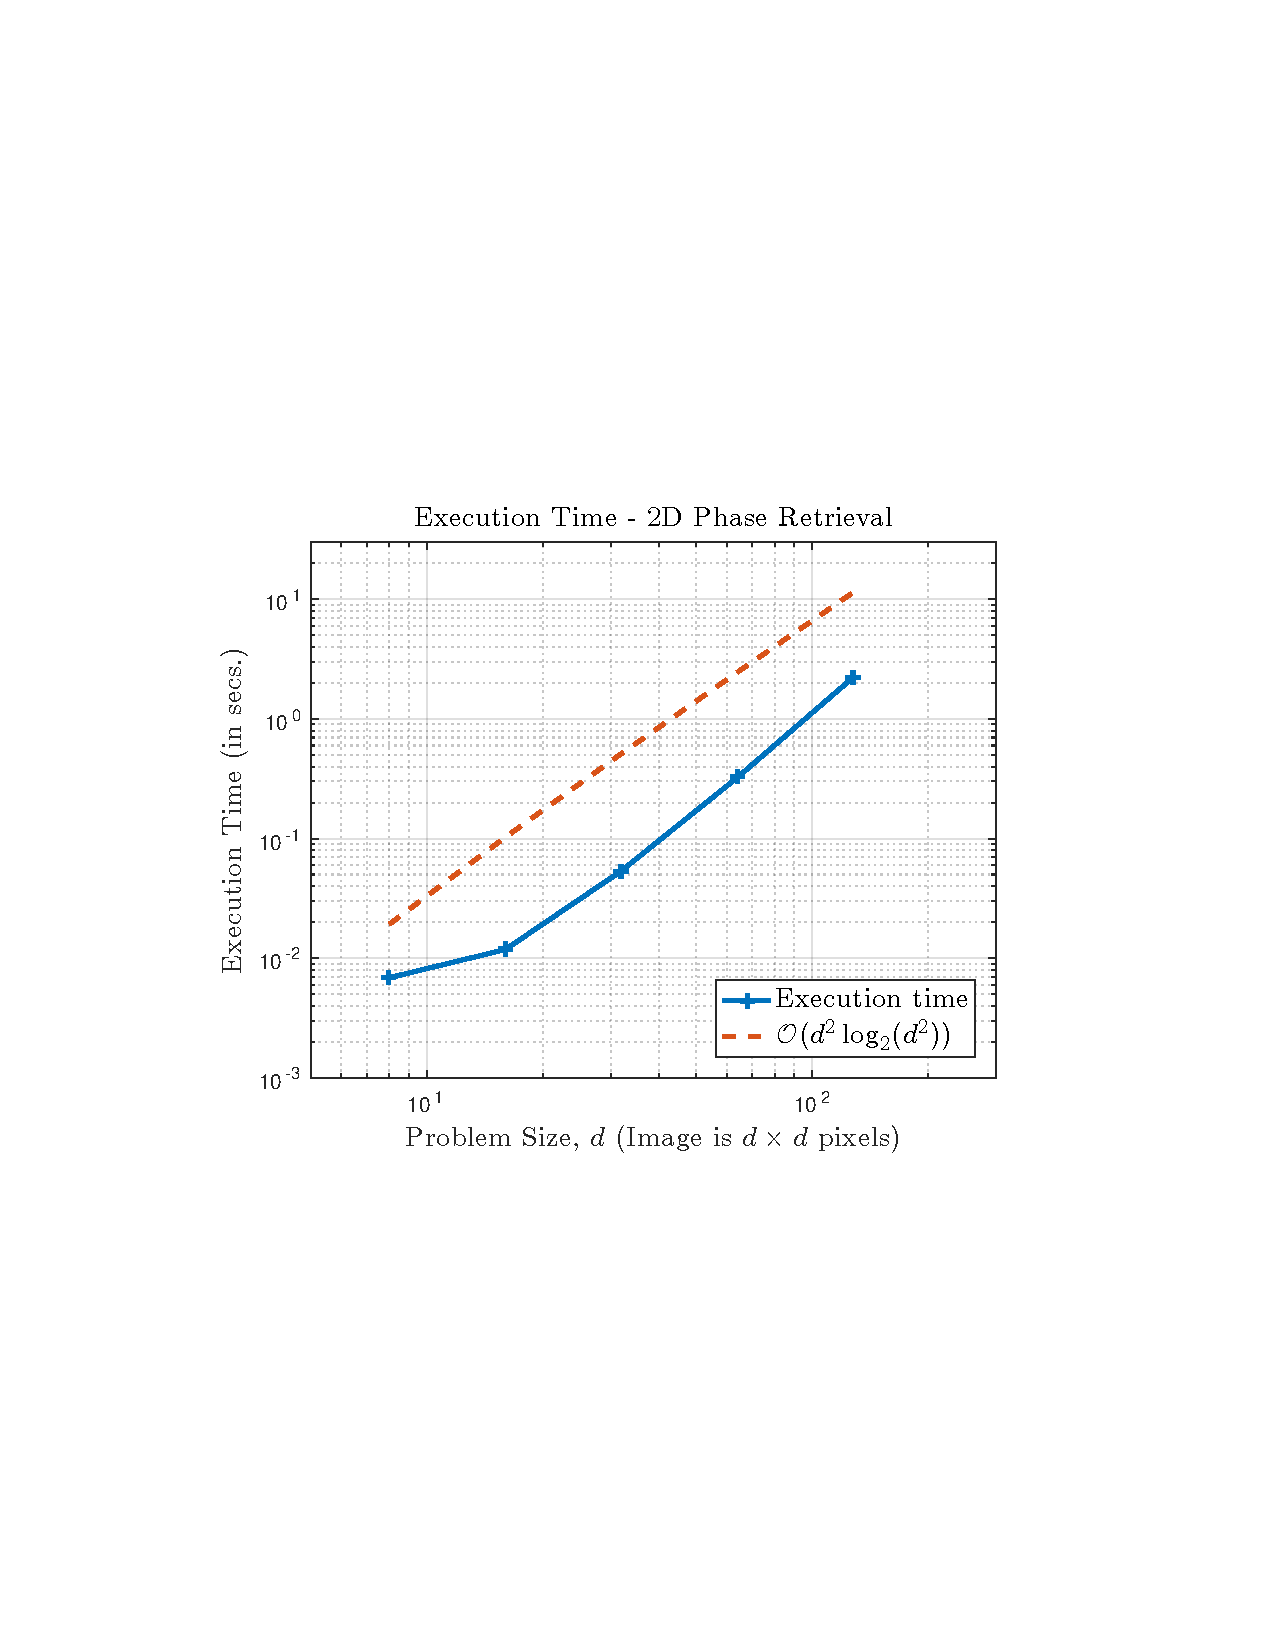
\includegraphics[clip=true, trim = 1.10in 3.25in 0.75in 3.25in,scale=0.55]{2d_figs/etime}
        \caption{Execution Time vs Problem Size}
        \label{fig:etime}
    \end{subfigure}
    \hfill
    \begin{subfigure}{0.495\textwidth}
        \centering
        %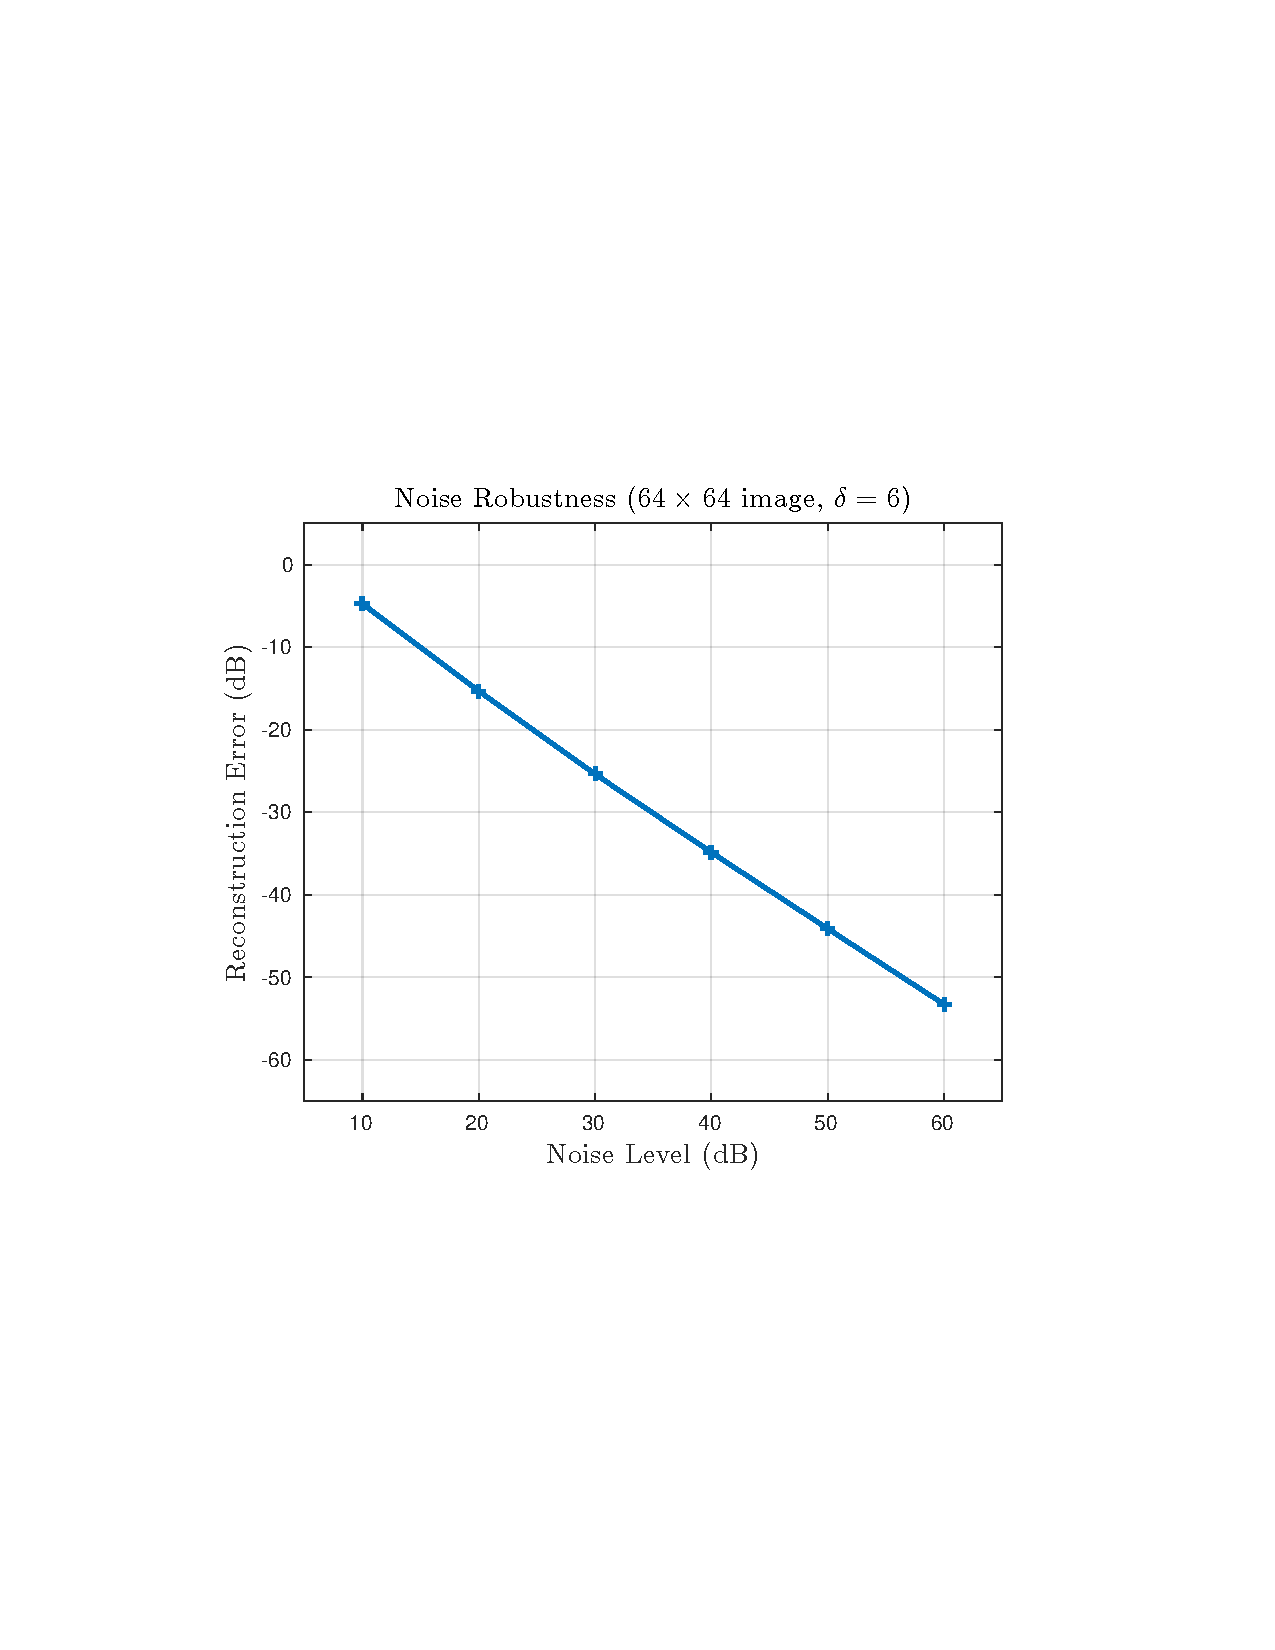
\includegraphics[clip=true, trim = 1.10in 3.15in 0.75in 3in,scale=0.55]{2d_figs/noise}
        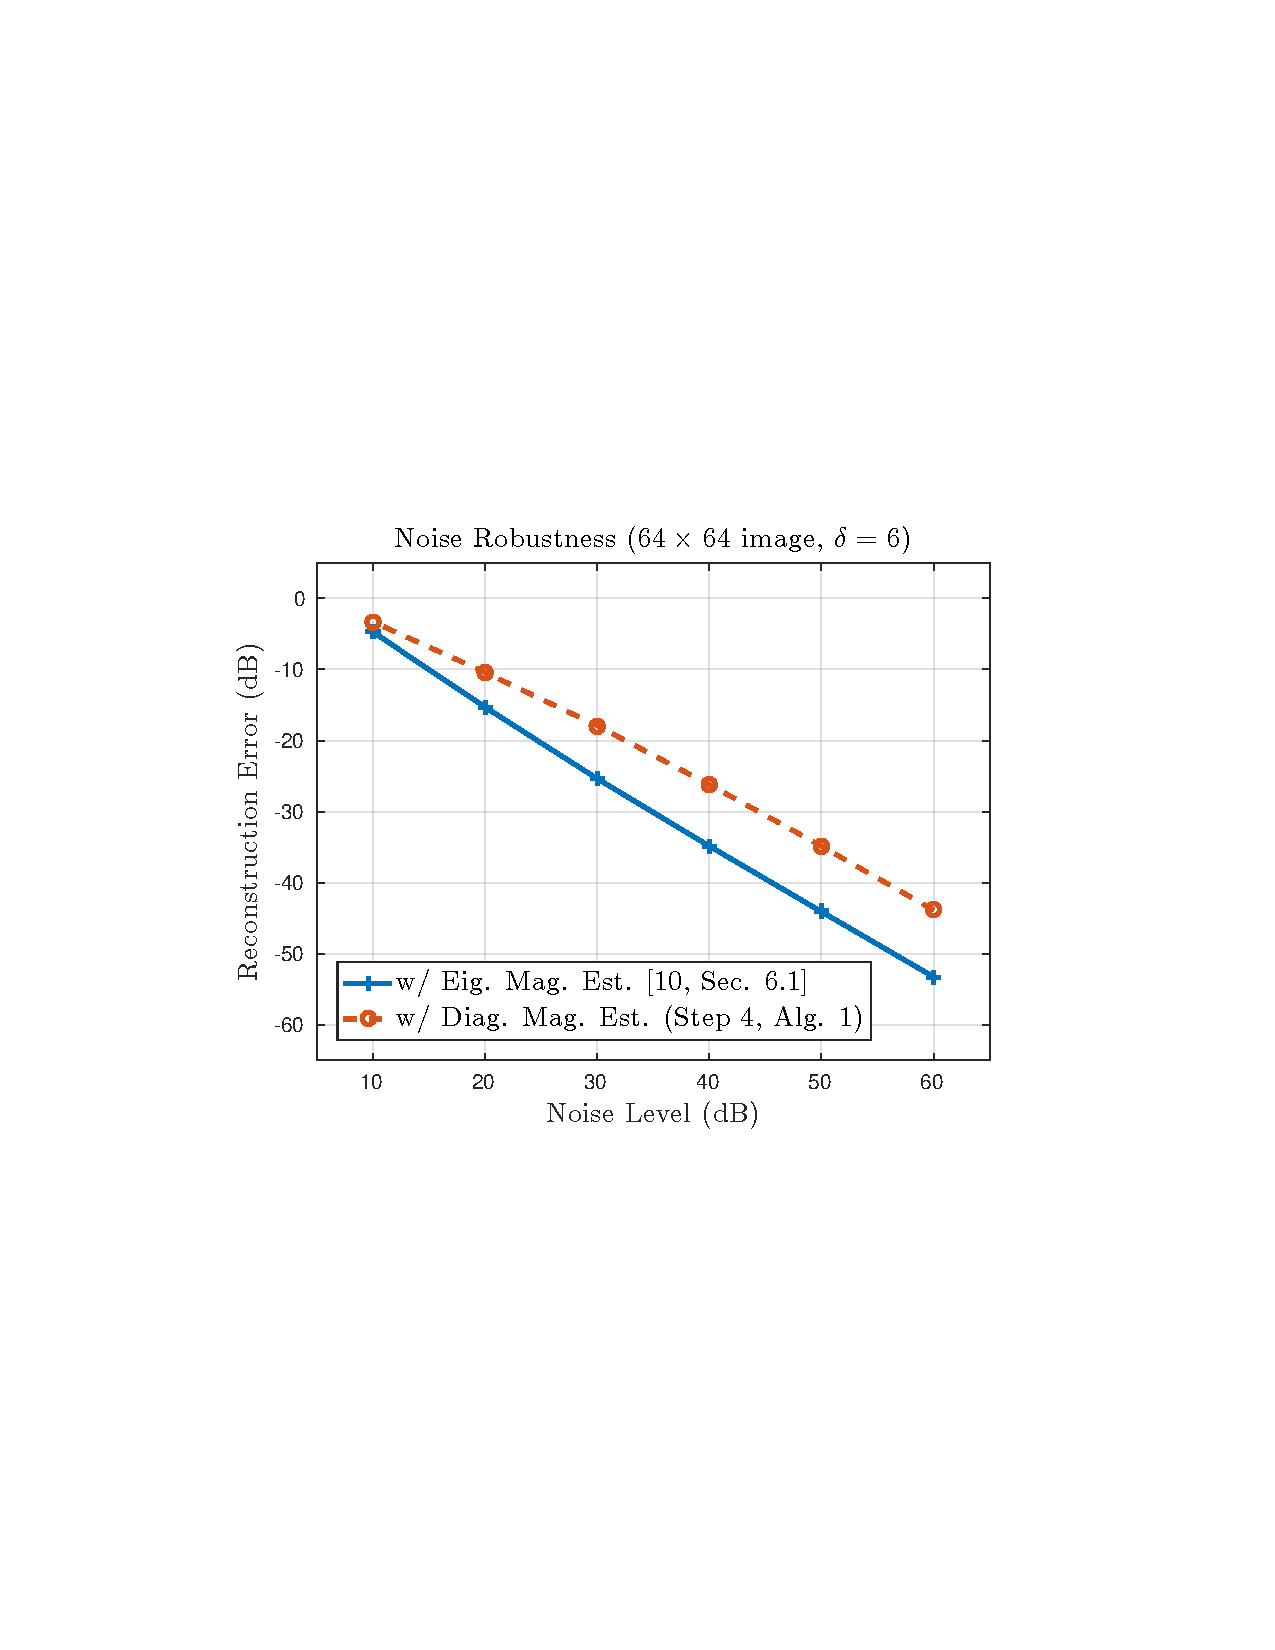
\includegraphics[clip=true, trim = 1.10in 3.25in 0.75in 3in,scale=0.575]{2d_figs/noise_alt}
        \caption{Noise Robustness of the Proposed Method}
        \label{fig:noise}
    \end{subfigure} 
    \vspace{0.05in}
    \caption{Evaluating the Efficiency and Robustness of the Proposed Two Dimensional Phase
    Retrieval Algorithm.}
    \label{fig:perf}
\end{figure}
%


\section*{Acknowledgments} % equivalent to \section*{ACKNOWLEDGMENTS}       
 
This work was supported in part by NSF DMS-1416752.% References

\section{Recovery Guarantees for 2D Phase Retrieval}
\label{sec:2d_recov}
In this section, we synthesize the results of \cref{ch:base_model,sec:2d_method} to produce guarantees of the robustness of \cref{alg:2d_pr} of the type presented in \cref{sec:recov_guar}.  We begin with a few lemmas that help us reduce the 2D phase retrieval problem in such a way that permits us to import some of the results we have proven in the 1D case.  First of all, we establish the relationship between the 2D measurement operator $\Mc$ defined in \eqref{eq:2d_meas_op} and its 1D analog, defined in \eqref{eq:meas_op}.

\begin{proposition}
  Fix $d, \delta \in \N$ such that $D := 2 \delta - 1 \le d$, and let $\{m_j\}_{j \in [D]}$ be a spanning family of masks.  Then setting $\a_u = \b_u = m_u, u \in [D]$, and letting $\Mc : T_\delta(\C^{d^2 \times d^2}) \to \R^{[d]_0^2 \times [D]^2}$ and $\Ac : T_\delta(\Cdxd) \to \R^{[d]_0 \times [D]}$ be as defined in \eqref{eq:2d_meas_op} and \eqref{eq:meas_op}.  Then $\sigma_{\max}(\Mc) = \sigma_{\max}^2(\Ac), \sigma_{\min}(\Mc) = \sigma_{\min}^2(\Ac),$ and $\kappa(\Mc) = \kappa(\Ac)^2$.
  \label{prop:2d_kron}
\end{proposition}

\begin{proof}[Proof of \cref{prop:2d_kron}]
  The definition of the tensor power of a linear operator stipulates that, for linear operators $A_1 : V_1 \to W_1, A_1 : V_1 \to W_1, B : V_1 \kron V_2 \to W_1 \kron W_2$, we have that $B = A_1 \kron A_2$ iff $B(u \kron v) = A_1(u) \kron A_2(v)$ for all $u, v \in V$.  If we identify $\B(\C^{d^2 \times d^2})$ with $(T_\delta(\Cdxd))^{\kron 2}$ and $\R^{[d]_0^2 \times [D]^2}$ with $(\R^{[d]_0 \times [D]})^{\kron 2}$, then we claim that $\Mc = \conj{\Ac} \kron \Ac$.  Indeed, from \eqref{eq:2d_meas_op} we can see that, for $U, V \in T_\delta(\Cdxd)$, we have
  \begin{align*}
    \Mc(U \kron V)_{(\ell, \ell', u, v)} &= \inner{U \kron V, S_{\ell'} \conj{m_u}\conj{m_u}^* S^*_{\ell'} \kron S_\ell m_v m_v^* S^*_\ell} \\
    &= \inner{U, S_{\ell'} \conj{m_u}\conj{m_u}^* S^*_{\ell'}} \inner{V, S_\ell m_v m_v^* S^*_\ell},
  \end{align*}
  while
  \begin{align*}
    (\conj{\Ac(U)} \kron \Ac(V))_{(\ell, \ell', u, v)} &= \conj{\Ac(U)}_{(\ell, u)} \kron \Ac(V)_{(\ell', v)} \\
    &= \inner{U, S_{\ell'} \conj{m_u}\conj{m_u}^* S^*_{\ell'}} \inner{V, S_\ell m_v m_v^* S^*_\ell},
  \end{align*}
  which proves the claim.  To finish the proposition, we simply observe that the singular values of $\Mc$ are therefore the products of the singular values of $\Ac$ and $\conj{\Ac}$, which include $\sigma_{\min}(\Ac)^2$ and $\sigma_{\max}(\Ac)^2$ as extrema.
\end{proof}

\Cref{lem:2d_diag_kron} states a similar result regarding the process by which the main diagonal is extracted from the measurements.
\begin{lemma}
  With notation as in \cref{prop:2d_kron,prop:mag_est_imp}, we have that \[\kappa(P_{\diag(\C^{d^2 \times d^2}, 0)} \circ \Mc^{-1}) = \kappa(P_{\diag(\Cdxd, 0)} \circ \Ac)^2.\]
  \label{lem:2d_diag_kron}
\end{lemma}
\begin{proof}[Proof of \cref{lem:2d_diag_kron}]
  This comes immediately from observing that $P_{\diag(\C^{d^2 \times d^2}, 0)} = P_{\diag(\Cdxd, 0)}^{\kron 2}$ and citing the fact that $\Mc^{-1} = \conj{\Ac}^{-1} \kron \Ac^{-1}$ (as shown in the proof of \cref{prop:2d_kron}).
\end{proof}

\Cref{prop:2d_specgap} establishes the spectral gap of the 2D analog of the graph $G$ used in the angular synchronization step in line 3 of \cref{alg:2d_pr}, which will allow us to use results from \cref{sec:Perturb} and \cref{ch:ang_sync}.
\begin{proposition}
  Let $G = (V = [d]^2, E)$ be the unweighted graph whose adjacency matrix is given by $W = \B(\one_{d^2} \one_{d^2}^*) - I_{d^2}$, and let $D = \diag(W \one_{d^2})$ be the degree matrix of $G$.  Then $\tau_G = \lambda_2(D - W)$, the spectral gap of $G$ and the second smallest eigenvalue of $D - W$, is given by $(2 \delta - 1) \tau_{\rm 1D} = \bigO(\delta^4 / d^2)$, where $\tau_{\rm 1D} > \frac{\pi^2}{3}\frac{\delta^3}{d^2}$ is the spectral gap of the matrix described in \cref{lem:EigGap}.
  \label{prop:2d_specgap}
\end{proposition}

\begin{proof}[Proof of \cref{prop:2d_specgap}]
  Recognizing that $\one_{d^2} = \one_d^{\kron 2}$, we calculate that
  \begin{align*}
    W \one_{d^2} &= (T_\delta(\one_d \one_d^*))^{\kron 2} \one_{d^2} - \one_{d^2} = (T_\delta(\one_d \one_d^*) \one_d)^{\kron 2} - \one_{d^2} \\
    &= ((2 \delta - 1) \one_d)^{\kron 2} - \one_{d^2} = ((2 \delta - 1)^2 - 1) \one_{d^2},
  \end{align*}
  so that $D = ((2 \delta - 1)^2 - 1) I_{d^2}$.  Therefore, by \cref{thm:Factorized_P11}, \[D - W = (2 \delta - 1)^2 I_{d^2} - (T_\delta(\one_d \one_d^*))^{\kron 2} = F_d^{\kron 2} ((2 \delta - 1)^2 I_{d^2} - \Lambda^{\kron 2}) (F_d^*)^{\kron 2},\] where $\Lambda$ is the diagonal matrix of $T_\delta(\one_d \one_d^*)$'s eigenvalues, as in \cref{lem:spectrum}.  The conclusion of the proposition is then immediate: \[\tau_G = (2 \delta - 1)^2 - \lambda_{d^2 - 1}(\Lambda^{\kron 2}) = (2 \delta - 1)^2 - (2 \delta - 1) \lambda_{d - 1}(\Lambda) = (2 \delta - 1) \tau_{\rm 1D}.\]
\end{proof}
The following lemma is a minor variant of \eqref{eq:empty_rho} of \cref{lem:EtaBound}.
\begin{lemma}
  Suppose $X, X_0 \in \Cmxn$ have the same support set $\Ic \subset [m] \times [n]$ and $\min_{(j, k) \in \Ic} \abs{(X_0)_{jk}} \ge a > 0$.  Then if we define \[\tX_{ij} = \begin{piecewise} \sgn(X_{ij}) & (i, j) \in \Ic \\ 0 & \ow \end{piecewise}\] and $\tX_0$ similarly, we have \[\norm{\tX - \tX_0}_F \le \frac{2 \norm{X - X_0}_F}{a}\]
  \label{lem:2d_srho}
\end{lemma}

\begin{proof}[Proof of \cref{lem:2d_srho}]
  We set $N = X - X_0$ and follow the argument of \eqref{eq:srho_b1} to see that, for $(j, k) \in \Ic$, \[\abs{(\tX_0)_{jk} - \tX_{jk}} \le 2 \dfrac{\abs{N_{jk}}}{\abs{(X_0)_{jk}}} \le 2 \dfrac{\abs{N_{jk}}}{a}.\]  The proof is complete by squaring both sides and summing over $\Ic$.
\end{proof}

\begin{algorithm}[htbp]
\renewcommand{\algorithmicrequire}{\textbf{Input:}}
\renewcommand{\algorithmicensure}{\textbf{Output:}}
\caption{2D Phase Retrieval, Improved Angular Synchronization}
\label{alg:2d_pr_wang}
\begin{algorithmic}[1]
    \REQUIRE Measurements $\y = \Mc(\mathbf{Q}) + n \in \R^{d^2 D^2}$ and masks $\a_u, \b_v$ as per \eqref{def:Measurements}
    \ENSURE $X \in \C^{d \times d}$ with $X \approx \eit Q$ for some $\theta \in [0, 2 \pi]$ 
    \STATE Compute the Hermitian matrix $P = \Big( \left(\mathcal{M} \big|_{\mathcal{P}}\right)^{-1} {\bf y}\Big)/2 + \Big( \left(\Mc \big|_{\mathcal{P}}\right)^{-1} {\bf y}\Big)^*/2  \in \mathcal{P}\left(\mathbbm{C}^{d^2\times d^2}\right)$ as an estimate of $\mathcal{P} \left( \mathbf{Q} \right)$.  $\mathcal{M}$ and $\mathcal{P}$ are as defined in \eqref{eq:2d_meas_op} and \S\ref{sec:linear}.
    \STATE Form the matrix of phases, $\widetilde{P} \in \mathcal{P}\left(\mathbbm{C}^{d^2\times d^2}\right)$, by normalizing the non-zero entries of $P$.
    \STATE Compute the solution $\hZ$ to \eqref{eq:ang_sync_sdp} with $L = (2 \delta - 1)^2 I_{d^2} - \widetilde{P}$.  Set $U = \sgn(\mat_{(d, d)} Z)$ to be the estimate of the phases of $Q$, where $Z$ is the top eigenvector of $\hZ$.
    \STATE Use the diagonal entries of $P$ to compute $M_{j,k} \approx \left| Q_{j,k} \right|^2$ for all $j,k \in [d]$ as per \S\ref{sec:Getmags}.
    \STATE Set $X_{j,k} = \sqrt{M_{j,k}} \cdot U_{j,k}$ for all $j,k \in [d]$ to form $X$
    %\STATE Set $\x = W^* \widetilde{\x}$ 
    \end{algorithmic}
\end{algorithm}

Synthesizing the results in this section, we may give a complete error bound for 2D phase retrieval.  We note that this uses the improved angular synchronization method proposed in \cref{ch:ang_sync}.  Although the numerical analysis in \cref{sec:2d_num} was completed using \cref{alg:2d_pr} (since the eigenvector-based angular synchronization is significantly cheaper and roughly as accurate, empirically), we present \cref{alg:2d_pr_wang} here for reference in \cref{thm:2d_recov}.

\begin{theorem}
  Suppose that $\{m_j\}_{j \in [D]} \subset \Cd$ is a local measurement system with support $\delta$ satisfying $D = 2 \delta - 1 \le d$, and define $\Mc$ as in \eqref{def:Measurements} with $\a_u = \b_u = m_u, u \in [D]$.  $Q$ is the ground truth objective image, and we set $\mathbf{Q} := \mathbf{Q}$.  Supposing further that line 3 of \cref{alg:2d_pr_wang} solves \eqref{eq:ang_sync} exactly, then the output $X$ satisfies
  \begin{equation}
    \begin{aligned}
      \mintheta \norm{X - \eit Q}_F &\le \frac{16}{5} \dfrac{\norm{\vec Q}_\infty}{\abs{\vec Q}_{\min}^2} \left(\dfrac{d}{\delta^2}\right) \sigma_{\min}^{-1}(\Mc) \norm{n}_2 + d^{1/2} \sqrt{\sigma_{\min}^{-1}(\Mc) \norm{n}_2} \\
      \mintheta \norm{X - \eit Q}_F &\le \frac{16}{5} \dfrac{\norm{\vec Q}_\infty}{\abs{\vec Q}_{\min}^2} \left(\dfrac{d}{\delta^2}\right) \kappa(\Mc) \frac{\norm{\B(\mathbf{Q})}_F}{\SNR} \\ &\quad + d^{1/2} \sqrt{\kappa(\Mc) \frac{\norm{\B(\mathbf{Q})}_F}{\SNR}} \\
    \end{aligned}
    \label{eq:2d_recov}
  \end{equation}
  Using $\gamma_{\rm flat}$ with $a_\delta$ as in \cref{prop:nearflat_more}, the second inequality becomes
  \[\mintheta \norm{X - \eit Q}_F \le \frac{5}{2} \dfrac{d \norm{\vec Q}_\infty}{\abs{\vec Q}_{\min}^2} \frac{\norm{\B(\mathbf{Q})}_F}{\SNR} \quad + d^{1/2} (1 + \frac{18}{\delta - 1}) \sqrt{\frac{\norm{\B(\mathbf{Q})}_F}{\SNR}}\]
  \label{thm:2d_recov}
\end{theorem}

\begin{proof}[Proof of \cref{thm:2d_recov}]
  We begin by splitting up $\norm{X - \eit Q}_F$ into ``phase error'' and ``magnitude error'' terms, by writing \[\mintheta \norm{X - \eit Q}_F \le \mintheta \norm{\abs{Q} \circ (\sgn(X) - \eit \sgn(Q))}_F + \norm{\abs{X} - \abs{Q}}_F,\] and the second term is immediately bounded by $(d^2)^{1/4} \sqrt{\sigma_{\min}^{-1}(\Mc) \norm{n}_2}$ by quoting \cref{lem:diag_mag_diff}.  To get the first term, we bound \[\norm{\abs{Q} \circ (\sgn(X) - \eit \sgn(Q))}_F \le \norm{\vec Q}_\infty \norm{\sgn(X) - \eit \sgn(Q)}_F\] and quote \cref{lem:2d_srho} to get, for $\widetilde{P}$ as defined as in line 2 of \cref{alg:2d_pr_wang}, \[\norm{\widetilde{P} - \sgn{\mathbf{Q}}}_F \le \frac{2 \sigma_{\min}^{-1}(\Mc) \norm{n}_2}{\abs{\vec Q}_{\min}^2}.\]  We combine this with \cref{thm:improved_spec_pert}, using $\tau_G \ge \frac{\pi^2}{3}\frac{\delta^4}{d^2}$ from \cref{prop:2d_specgap}, to get \[\norm{\sgn(X) - \eit \sgn(Q)}_F \le \dfrac{2 \sqrt{2} \norm{\widetilde{P} - \sgn{\mathbf{Q}}}_F}{\sqrt{\tau_G}},\] and combining these gives \[\norm{\abs{Q} \circ (\sgn(X) - \eit \sgn(Q))}_F \le \dfrac{\norm{\vec Q}_\infty}{\abs{\vec Q}_{\min}} \dfrac{4 \sqrt{2} \sigma_{\min}^{-1}(\Mc) \norm{n}_2}{\sqrt{\frac{\pi^2}{3} \frac{\delta^4}{d^2}}},\] and we combine the constants to obtain \eqref{eq:2d_recov}.  The reduction in the case of $\gamma_{\rm flat}$ comes from \cref{prop:nearflat_more,prop:mag_est_imp}.
\end{proof}


\section*{Acknowledgement of joint authorship}

\Crefrange{sec:2d_intro}{sec:2d_num}, in full, are a reprint of material published with Mark Iwen, Rayan Saab, and Aditya Viswanathan in the Proceedings of SPIE vol.~10394, 2017.  \emph{Phase retrieval from local measurements in two dimensions}.  Available online as of 24 August 2017.
